\scanpage{126}

\[
\left.\begin{aligned}
\alpha\in B_{\unsure{n(p)|p}}&=\mathbb Z[\deleted{T}U]/\deleted{\unsure{\Phi}}F_p(U)\\
\zeta\in A_p&=\mathbb Z[T]/\Phi_p(T)
\end{aligned}\right|\quad\text{normaux}\qquad p\text{ premier impair}
\]

ils sont étales sur $\mathbb Z$ en les \deleted{$\unsure{p}$} $\ell\in\operatorname{Spec}(\mathbb Z)$, $\ell\ne p$ car en ces pts les racines de $F_p,\Phi_p$ sont distinctes.

Ramifiés en $\ell=p$ (une seule racine en \unsure{corps|carps} de car $p$)

\[
(\zeta-1)^{p-1}\equiv0\quad(p)\qquad\text{dans }A_{\deleted{\unsure{(p)}}}=A_{(p)}
\]

\[
\deleted{\unsure{1+T+\cdots}}\quad\zeta^{p-1}-(p-1)\zeta^{p-2}+\frac{(p-1)(p-2)}2\zeta^{p-3}-\ldots\ \deleted{\unsure{p}}\ 1
\]

\[
\deleted{1+T+\ldots+T^{p-1}\equiv(T-1)^{p-1}\quad(p)}
\]

\[
\begin{aligned}
(\zeta-1)^{p-1}&=(\zeta-1)^{p-1}-F_p(\zeta)\\
&=p\zeta^{p-2}+\left(\frac{(p-1)(p-2)}2-1\right)\zeta^{p-\deleted{2}\inserted{3}}+
\left(-\frac{(p-1)(p-2)(p-3)}6-1\right)\zeta^{p-4}\ldots
\end{aligned}
\]

\figure{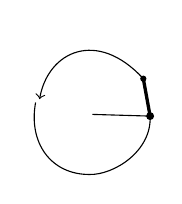
\begin{tikzpicture}[x=.72cm,y=.72cm]
\draw (1.02,0).. controls (1.05,-.62) and (.38,-1.04) ..(-.05,-1.03).. controls (-.74,-1.03) and (-1.13,-.46) ..(-1,.24);
\draw[->] (.90,.66).. controls (.08,1.55) and (-.78,1.14)..(-.93,.30);
\draw (0,.03)--(1.02,0);\draw[very thick] (1.02,0)--(.90,.66);\fill (1.02,0) circle (.07) (.90,.66) circle (.055);
\end{tikzpicture}}

\[
\frac1p(\zeta-1)^{p-1}=\zeta^{p-2}+
\]

\[
\begin{aligned}
N\left(\frac1p(\zeta-1)^{p-1}\right)&=\frac1{p^{p-1}}N(\zeta-1)^{p-1}.\\
N(\zeta-1)&=\prod_1^{p-1}(\zeta_i-1)=\deleted{\unsure{\prod|\varepsilon}}\cdot\prod(1-\zeta_i)=F_p(1)=\underbrace{1\ldots+1}=p\\
N\left(\frac1p(\zeta-1)^{p-1}\right)&=1
\end{aligned}
\]

\[
\boxed{(\zeta-1)^{p-1}=pu}\qquad u\ \text{\uline{unité}}
\]

Donc $(\zeta-1)A\supset pA$ \deleted{$\unsure{(\zeta-1|(\zeta-1)}$} donc

\[
\begin{aligned}
A/(\zeta-1)A&=(\underbrace{A/pA}_{A_0})/(\zeta-1)A_0=\bigl(\mathbb F_p[T]/(T-1)^{p-1}\bigr)/(T-1)\\
&=\mathrm F_p
\end{aligned}
\]

Donc $(\zeta-1)A$ est un idéal \uline{maximal}

% archive sheet number: 125
